\documentclass[../../main.tex]{subfiles}
\begin{document}

{\bf [解答]}

\begin{figure}[htb]
  \centering
  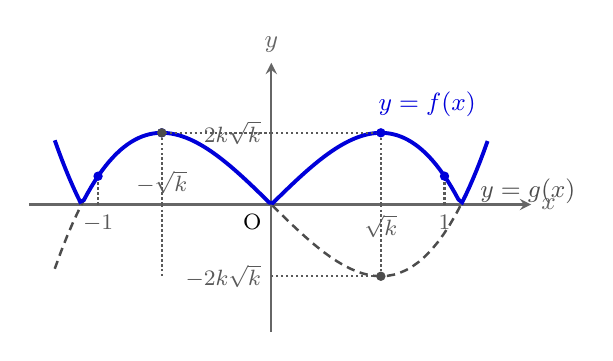
\begin{tikzpicture}[x=2.2cm, y=1.8cm, >=stealth,
    every node/.style={font=\small}]
    \def\kVal{0.4}
    \def\sqrtk{0.6325}
    \def\twoKsqrtK{0.5060}
    \def\fOne{0.2}

    % 座標軸
    \draw[->, thick, gray!80!black] (-1.4, 0) -- (1.5, 0) node[right] {$x$};
    \draw[->, thick, gray!80!black] (0, -0.9) -- (0, 1.0) node[above] {$y$};
    \node[below left, font=\footnotesize] at (0, 0) {$\mathrm{O}$};

    % y = g(x) (破線)
    \draw[densely dashed, line width=0.9pt, gray!60!black, domain=-1.25:1.25, samples=70]
    plot (\x, {\x*\x*\x - 3*\kVal*\x});

    % y = f(x) = |g(x)| (太実線)
    \draw[line width=1.4pt, blue!85!black, domain=-1.25:1.25, samples=120]
    plot (\x, {abs(\x*\x*\x - 3*\kVal*\x)});

    % 補助線
    \draw[densely dotted, thick, gray!70!black]
    (\sqrtk, 0) node[below, font=\footnotesize] {$\sqrt{k}$}
    -- (\sqrtk, \twoKsqrtK)
    -- (0, \twoKsqrtK) node[left, font=\footnotesize] {$2k\sqrt{k}$};
    \draw[densely dotted, thick, gray!70!black]
    (\sqrtk, 0)
    -- (\sqrtk, -\twoKsqrtK)
    -- (0, -\twoKsqrtK) node[left, font=\footnotesize] {$-2k\sqrt{k}$};

    \draw[densely dotted, thick, gray!70!black]
    (-\sqrtk, 0) node[above, font=\footnotesize] {$-\sqrt{k}$}
    -- (-\sqrtk, \twoKsqrtK)
    -- (0, \twoKsqrtK);
    \draw[densely dotted, thick, gray!70!black]
    (-\sqrtk, 0)
    -- (-\sqrtk, -\twoKsqrtK);

    \draw[densely dotted, thick, gray!70!black]
    (1, 0) node[below, font=\footnotesize] {$1$}
    -- (1, \fOne);
    \draw[densely dotted, thick, gray!70!black]
    (-1, 0) node[below, font=\footnotesize] {$-1$}
    -- (-1, \fOne);

    % 代表点
    \node[circle, fill=blue!85!black, inner sep=1.2pt] at (\sqrtk, \twoKsqrtK) {};
    \node[circle, fill=blue!85!black, inner sep=1.2pt] at (-\sqrtk, \twoKsqrtK) {};
    \node[circle, fill=gray!60!black, inner sep=1.2pt] at (\sqrtk, -\twoKsqrtK) {};
    \node[circle, fill=gray!60!black, inner sep=1.2pt] at (-\sqrtk, \twoKsqrtK) {};
    \node[circle, fill=blue!85!black, inner sep=1.2pt] at (1, \fOne) {};
    \node[circle, fill=blue!85!black, inner sep=1.2pt] at (-1, \fOne) {};

    % ラベル
    \node[above, font=\small, blue!85!black] at (0.9, 0.55) {$y=f(x)$};
    \node[below right, font=\small, gray!60!black] at (1.15, 0.25) {$y=g(x)$};
  \end{tikzpicture}
  \caption{$y=g(x)$ および $y=f(x)$ の概形（$0<k<1$ の例）}
  \label{fig:graph_gx_fx}
\end{figure}

$g(x)=x^3-3kx$とおくと$f(x)=|g(x)|$である．
$g(x)$は奇関数だからなので$f(x)$は偶関数である．故に$0\le x$で考える．
$g(x)$の一階微分は
\begin{align}
  g'(x)=3(x^2-k)
\end{align}
だから，$k$の大きさに応じて$g(x)$は挙動を変える．
以下これを個別に検討する．

\subparagraph{(i)$k\le0$の時}

この時は$g(x)$の増減表は以下のようになる．

\begin{table}[htb]
  \centering
  \caption{$k\le 0$ のときの $g(x)$ の増減表}
  \label{tab:variation_k_le_0}
  \begin{tabular}{c|c|c|c}
    $x$ & $0$ & $\dots$ & $1$ \\ \hline
    $g'$ & & $+$ & \\ \hline
    $g$ & $0$ & $\nearrow$ & $|1-3k|$
  \end{tabular}
\end{table}

$g'(x)\ge0$だから$g(x)$は単調増加で
\begin{align}
  g(0)=0, \quad
  g(1)=|1-3k|\ge0
\end{align}
に注意して
\begin{align}
  M(k)=g(1)=|1-3k|
\end{align}
である．

\subparagraph{(ii)$0<k\le 1$の時}

この時は$g(x)$の増減表は以下のようになる．

\begin{table}[htb]
  \centering
  \caption{$0<k\le 1$ のときの $g(x)$ の増減表}
  \label{tab:variation_k_le_1}
  \begin{tabular}{c|c|c|c|c|c}
    $x$ & $0$ & $\dots$ & $\sqrt{k}$ & $\dots$ & $1$ \\ \hline
    $g' $     &   & $-$ & $0$ & $+$ & \\ \hline
    $g  $ $0$ & & $\searrow$ & & $\nearrow$ & $|1-3k|$
  \end{tabular}
\end{table}

従って$f(x)=|g(x)|$の最大値の候補は（(i)と同様にして$f(0)$は最大値の候補から除外できて）$x=\sqrt{k},1$であり，
\begin{align}
  M(k)&=\max\{f(0),f(\sqrt{k}),f(1)\} \\
  &=\max\{|1-3k|,2k\sqrt{k}\}
\end{align}
である．

\subparagraph{(iii)$1\le k$の時}

この時は$g(x)$の増減表は以下のようになる．

\begin{table}[htb]
  \centering
  \caption{$1\le k$ のときの $g(x)$ の増減表}
  \label{tab:variation_k_ge_1}
  \begin{tabular}{c|c|c|c}
    $x$ & $0$ & $\dots$ & $1$ \\ \hline
    $g' $ & & $-$ & \\ \hline
    $g  $ $0$ & & $\searrow$ & $1-3k|$
  \end{tabular}
\end{table}

故に(i)と同様にして，最大値は$x=1$の時であり
\begin{align}
  M(k)=f(1)=|1-3k|
\end{align}
である．
\casesend

以上をまとめて
\begin{align}
  M(k)=
  \begin{cases}
    |1-3k|&k\le0,1\le k \\
    \max\{|1-3k|,2k\sqrt{k}\}&0<k\le1
  \end{cases}
\end{align}
であるから，図示すると下図のようになる．

\begin{figure}[htb]
  \centering
  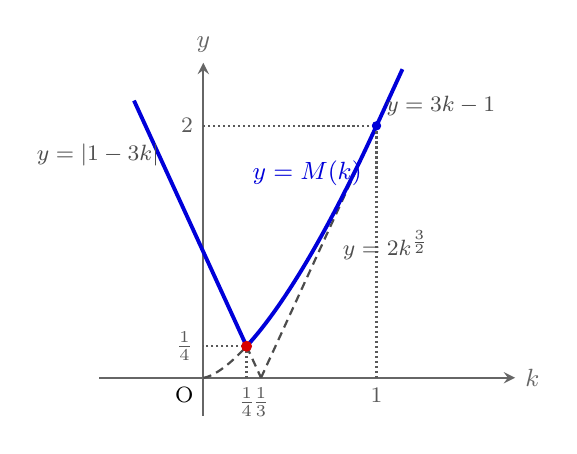
\begin{tikzpicture}[x=2.2cm, y=1.6cm, >=stealth,
    every node/.style={font=\small}]
    % 座標軸
    \draw[->, thick, gray!80!black] (-0.6, 0) -- (1.8, 0) node[right] {$k$};
    \draw[->, thick, gray!80!black] (0, -0.3) -- (0, 2.5) node[above] {$y$};
    \node[below left, font=\footnotesize] at (0, 0) {$\mathrm{O}$};

    % 補助延長線（比較用・破線）
    \draw[densely dashed, thick, gray!60!black, domain=0.25:0.3333] plot (\x, {1 - 3*\x});
    \draw[densely dashed, thick, gray!60!black, domain=0.3333:1] plot (\x, {3*\x - 1});
    \draw[densely dashed, thick, gray!60!black, domain=0:0.25, samples=30] plot (\x, {2*\x*sqrt(\x)});

    % M(k) の主曲線（太実線）
    % k <= 1/4: y = 1 - 3k
    \draw[line width=1.4pt, blue!85!black, domain=-0.4:0.25] plot (\x, {1 - 3*\x});
    % 1/4 <= k <= 1: y = 2 k^(3/2)
    \draw[line width=1.4pt, blue!85!black, domain=0.25:1, samples=50] plot (\x, {2*\x*sqrt(\x)});
    % k >= 1: y = 3k - 1
    \draw[line width=1.4pt, blue!85!black, domain=1:1.15] plot (\x, {3*\x - 1});

    % 代表点・垂線
    \draw[densely dotted, thick, gray!70!black] (0.25, 0) node[below, font=\footnotesize] {$\frac{1}{4}$}
    -- (0.25, 0.25)
    -- (0, 0.25) node[left, font=\footnotesize] {$\frac{1}{4}$};
    \draw[densely dotted, thick, gray!70!black] (0.3333, 0) node[below, font=\footnotesize] {$\frac{1}{3}$} -- (0.3333, 0);
    \draw[densely dotted, thick, gray!70!black] (1, 0) node[below, font=\footnotesize] {$1$}
    -- (1, 2)
    -- (0, 2) node[left, font=\footnotesize] {$2$};

    % 最小値の点（強調）
    \node[circle, fill=red!85!black, inner sep=1.4pt] at (0.25, 0.25) {};
    \node[circle, fill=blue!85!black, inner sep=1.2pt] at (1, 2) {};

    % 関数ラベル
    \node[above left, font=\footnotesize, gray!60!black] at (-0.2, 1.6) {$y=|1-3k|$};
    \node[right, font=\footnotesize, gray!60!black] at (0.75, 1.05) {$y=2k^{\frac{3}{2}}$};
    \node[above right, font=\footnotesize, gray!60!black] at (1.0, 2.0) {$y=3k-1$};
    \node[above, font=\small, blue!85!black] at (0.6, 1.45) {$y=M(k)$};
  \end{tikzpicture}
  \caption{$M(k)$ のグラフ}
  \label{fig:graph_Mk}
\end{figure}

故に求める最小値は
\begin{align}
  M\left(\dfrac{1}{4}\right)=\dfrac{1}{4}
\end{align}
である．$\cdots$(答)

\newpage

\end{document}
